\documentclass{article}
\usepackage{graphicx}
\usepackage[margin=1in]{geometry}
\usepackage{pdfpages}
\usepackage[colorlinks, urlcolor=blue]{hyperref}
\renewcommand{\familydefault}{\sfdefault}

\begin{document}
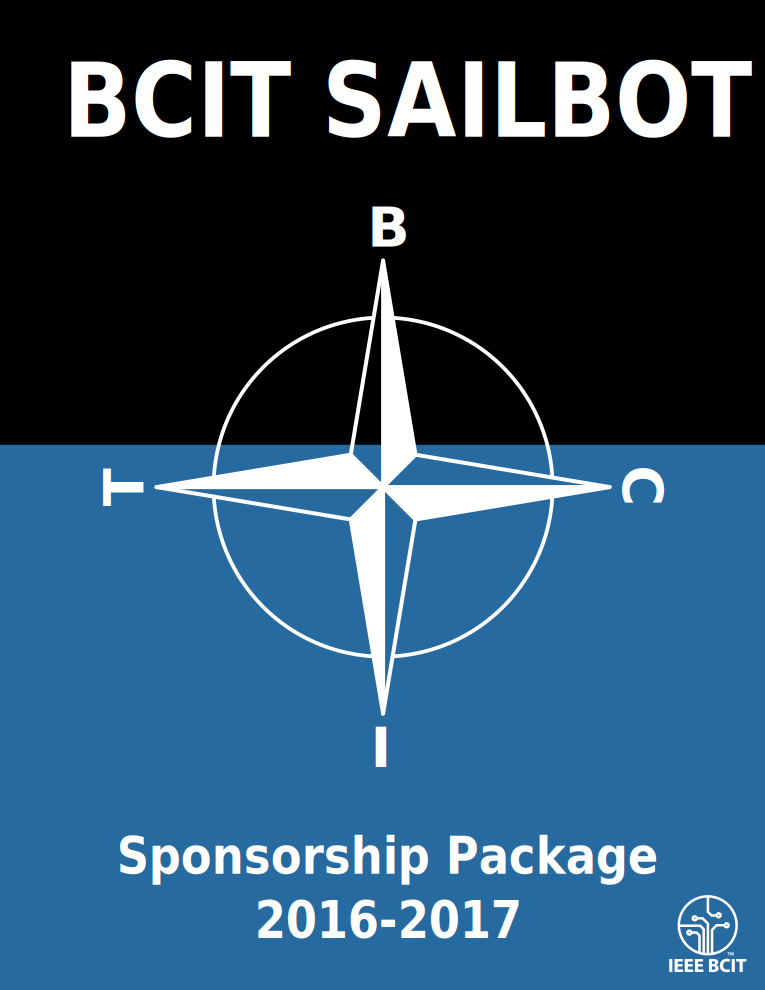
\includepdf{./images/frontPage.pdf}

\section*{Who We Are}
BCIT Sailbot is a student initiative under IEEE BCIT to design and build an
autonomous sailboat, or "sailbot" for the International Robotic Sailing Regatta 
(IRSR) in June 2017. This will be BCIT's first time competing and we intend to 
win.

Our team consists of over a dozen students that come from BCIT's Mechatronics, 
Electrical Engineering and Mechanical Engineering programs. These are students, 
who come together not for class credit or financial gain, but to further their 
abilities by being a part of a challenging project. Designing and builing the 
sailbot will help them improve both their technical, and non-technical skill 
sets as well as some MacGyvering skills like any good engineering project.

\section*{Sail What?}
A sailbot is an autonomous sailboat. By relying on the wind for propulsion, and 
using solar power to reliably power the entire craft we have a vehicle that is
well suited for long distance voyages.

Sailbots have great potential in applications such as fish stock management, 
environmental monitoring for the mining and petroleum industries and 
oceanography. It is a developing technology and competitions like the IRSR allow
students to take part in its advancement.

\section*{The Competition}
Every year teams from across the world come to compete at the International 
Robotic Sailing Regatta competition. At the IRSR, there are a number of races 
that test navigation, tactics and design. During the competiton, the saiboat 
must steer and trim sails based on measurements of the wind, position, and 
direction without human intervention. 

This year IRSR takes place in Annapolis, Maryland June 11 - 16th at the United 
States Naval Academy. 

If you'd like to check out the IRSR some more, their website is right 
\href{http://sailbot.org}{here}.

\section*{Why We Need Your Help}

More than anything else, developing a state of the art robotic sailboat requires 
dedication from the entire team. It also requires advanced materials, high-tech 
microcontrollers, accurate sensors and powerful communication equipment. These 
items are expensive, and this is why your support is so critical to the success 
of our team.

Sailbot Budget

Project Timeline 

Sponsorship Levels 

\section*{Contact Information}
If you would like further information regarding the BCIT Sailbot team, or
would like to show your support for the team, please contact us at
bcit.sailbot@gmail.com


Sincerely,

Matthew Knight,
BCIT Sailbot Team Captain

\end{document}
